% Template for ICASSP-2016 paper; to be used with:
%          spconf.sty  - ICASSP/ICIP LaTeX style file, and
%          IEEEbib.bst - IEEE bibliography style file.
% --------------------------------------------------------------------------
\documentclass[12pt]{article}
\usepackage{spconf, amsmath, graphicx, float}
\usepackage{scrlayer-scrpage}
\usepackage{subfig}
\usepackage{balance}
\clearpairofpagestyles
\cfoot*{\pagemark}
% Example definitions.
% --------------------
\def\x{{\mathbf x}}
\def\L{{\cal L}}

% Title.
% ------
\title{Movie Review Sentiment Analysis}
%
% Single address.
% ---------------
\name{{\bf Atom Group}: Jifu Zhao (jzhao59), Jinsheng Wang (jwang278)}
\address{Nuclear, Plasma, and Radiological Engineering \\
              University of Illinois at Urbana-Champaign\\
              Urbana, IL 61801}

\begin{document}
%\ninept
%
\maketitle

\section{Introduction}
\quad\ In this project, our goal is to build a model to predict the sentiment of a given movie review. The data was collected through the IMDB provided on Kaggle. The original training data set has 25,000 records and each record has 2 features, movie review and movie sentiment. The test data set also has 25,000 data set but only with one feature, movie review. In this project, we first explore the given training data set. After some pre-processing methods, we applied several different models to predict the chance of being positive/negative of a given movie review. More details will be described in the following sections.

\section{Pre-processing}
\quad\ As usual, the very first step is to load the data into memory for later processing. In our code, pandas DataFrame was used to simplify this task. We found that some original movies were retrieved from websites, containing html tags, thus BeatifulSoup4 package was used to clean off these tags. Moreover, numbers, which are barely useless in predicting movie sentiment, got removed by applying regular expression onto each  movie record. Lastly, all words were transformed into lower case and joined by white space for later tf-idf vector generation.\\

Tf-idf stands for term frequency - inverse document frequency, which is a widely used natural language processing technique for sentiment analysis and topic modelling. In our model, we filter words that showed up at least 3 times, removing stop words, counting both single-word and two-consecutive-word for up to 10000 features. The generated tf-idf matrix was then feed into different classifiers to learn prediction models.

In our Python code, besides pandas, bs4, re and numpy packages for data reading, writing and cleaning, we also loaded the widely used sklearn machine learning package to build models for sentiment prediction as in the code submitted.

\section{Methods}
\quad\  In this methods section, we built 6 different models to perform prediction, and average them with different weights to find the best additive model.

\subsection{Logistic Regression with Ridge Penalty}
\quad\ In our first model, Model 1, we used logistic regression classifier with L2 ridge penalty: LogisticRegression from sklearn.linear${\_}$model class. After cross validation, we set the C, representing the inverse of regularization strength to be 2.7825549 (C must be a positive float. Like in support vector machines, smaller values specify stronger regularization). The training AUC for this method was found to be 0.988545088.

\subsection{Logistic Regression with Lasso Penalty}
\quad\ In our second model, Model 2, we used logistic regression classifier with Lasso penalty: LogisticRegression from sklearn.linear${\_}$model class. After cross validation, we also set the C, representing the inverse of regularization strength to be 2.7825549 (C must be a positive float. Like in support vector machines, smaller values specify stronger regularization). The training AUC for this method was found to be 0.9879110592.

\subsection{Multinomial Naive Bayes Model}
\quad\ In our third model, Model 3, we used Multinomial Naive Bayes model classifier MultinomialNB from sklearn.naive${\_}$bayes. After cross validation, we set the alpha, representing the additive (Laplace/Lidstone) smoothing parameter  to be 5 (alpha default to be 1, 0 for no smoothing). The training AUC for this method was found to be 0.9498812928.

\subsection{AdaBoost}
\quad\ In our forth model, Model 4, we used AdaBoost model classifier AdaBoostClassifier from sklearn.ensemble. We first split the original training data into 3:1 train to test data for cross validation. After cross validation, we set the n${\_}$estimators, representing the maximum number of estimators at which boosting is terminated to be 400 and learning rate learning${\_}$rate to be 1.0 (default value). The training AUC for this method was found to be 0.9622484224.

\subsection{Gradient Boosting}
\quad\ In our fifth model, Model 5, we used gradient boosting model classifier GradientBoostingClassifier from sklearn.ensemble. We also first split the original training data into 3:1 train to test data for cross validation. After cross validation, we set the n${\_}$estimators, representing the maximum number of estimators at which boosting is terminated to be 500, learning rate learning${\_}$rate to be 0.2 (0.1 as default value), subsample to be 1. Other final parameters setting can be seen in Python file. The training AUC for this method was found to be 0.9919758208.

\subsection{Random Forest}
\quad\ In our last model, Model 6, we used random forest model classifier RandomForestClassifier from sklearn.ensemble. We also first split the original training data into 3:1 train to test data for cross validation. After cross validation, we set the n${\_}$estimators, representing the maximum number of estimators at which boosting is terminated to be 500. Other final parameters setting can be seen in Python file. The traning AUC for this method was found to be 1.0.

\section{Code Description}
\quad\ All of our code for part I is contained in the file named $mymain.py$. 

There are basically three parts in the Python file. At the very beginning, we loaded the necessary packages. In the second part of the code, we did data preprocessing: first read in the training and test data sets, then performed necessary data cleaning and built up tf-idf matrix. For the last part, we mainly built our 6 models as above. These built models will make predictions and the results are the added with certain ratio, finally saved into local file system as required by the project description.

Due to the amount of data and number of models we trained, the code needs a lot of time to run. As tested, the total running time is around 4 hours.

\section{Part I - Results}
\quad\ To evaluate our model, we used the metric described below:
\begin{equation}
AUC = \sum_{i=1}^6 w_{i} \cdot {AUC}_{i}
\end{equation}
where 6 is the total number of individual models, $i$ represents ith model. $ w_{i} $ is the weight of ith model to final additive model. Our final test score get from Kaggle is 0.95518.

\begin{table}[htb]
 \caption{Summary of Training/Testing AUC} \label{result}
\begin{center}
  \begin{tabular}{  c  c  c  c  c  c  c}
    \hline
    w1 & w2 & w3 & w4 & w5 & w6 \\ \hline
    2/8 & 2/8 & 1/8 & 1/8 & 1/8 & 1/8\\ \hline
  \end{tabular}
\end{center}
\end{table}

\balance
\section{Part II - Results}

\quad\ All of our code for part II is contained in the file named visualization.py. 

For this visualization part, in order to run the visualization work easy and fast, we simpliy used the average prediciton of logistic classsifier with lasso and ridge penalty. All words used were retrieved from the tf-idf vectorizer.  In order to define positive words and negative words, we first get the index by sorting feature coefficients and both lasso and ridge models, then filtered words corresponding to those index out. Then we select 200 most positive words and 200 most negative words from Lasso and Ridge model, then use the common words showed in both models as the final positive and negative words. So, finally we have 159 positive words and 155 negatives words as candidate for visualization purpose.

After having our positive/negative words vocabulary, we loop over each new movie review, first predict the sentiment using the above averaged model. For this part, we set review with score higher than 0.5 as positive sentiment with 1 and vice versa. After getting sentiment prediction, for each review, we color each word in the positive vocabulary with green and negative with pink. Based on TA's code, we present our visualization result as a html file implemented in Python, with example figures as shown below.
 
\subsection*{Acknowledgement}
\quad\ The authors would like to thank Xichen Huang for his tutorial notebook on Piazza and Kaggle website for data cleaning ideas provided online.

\begin{figure*}\centering
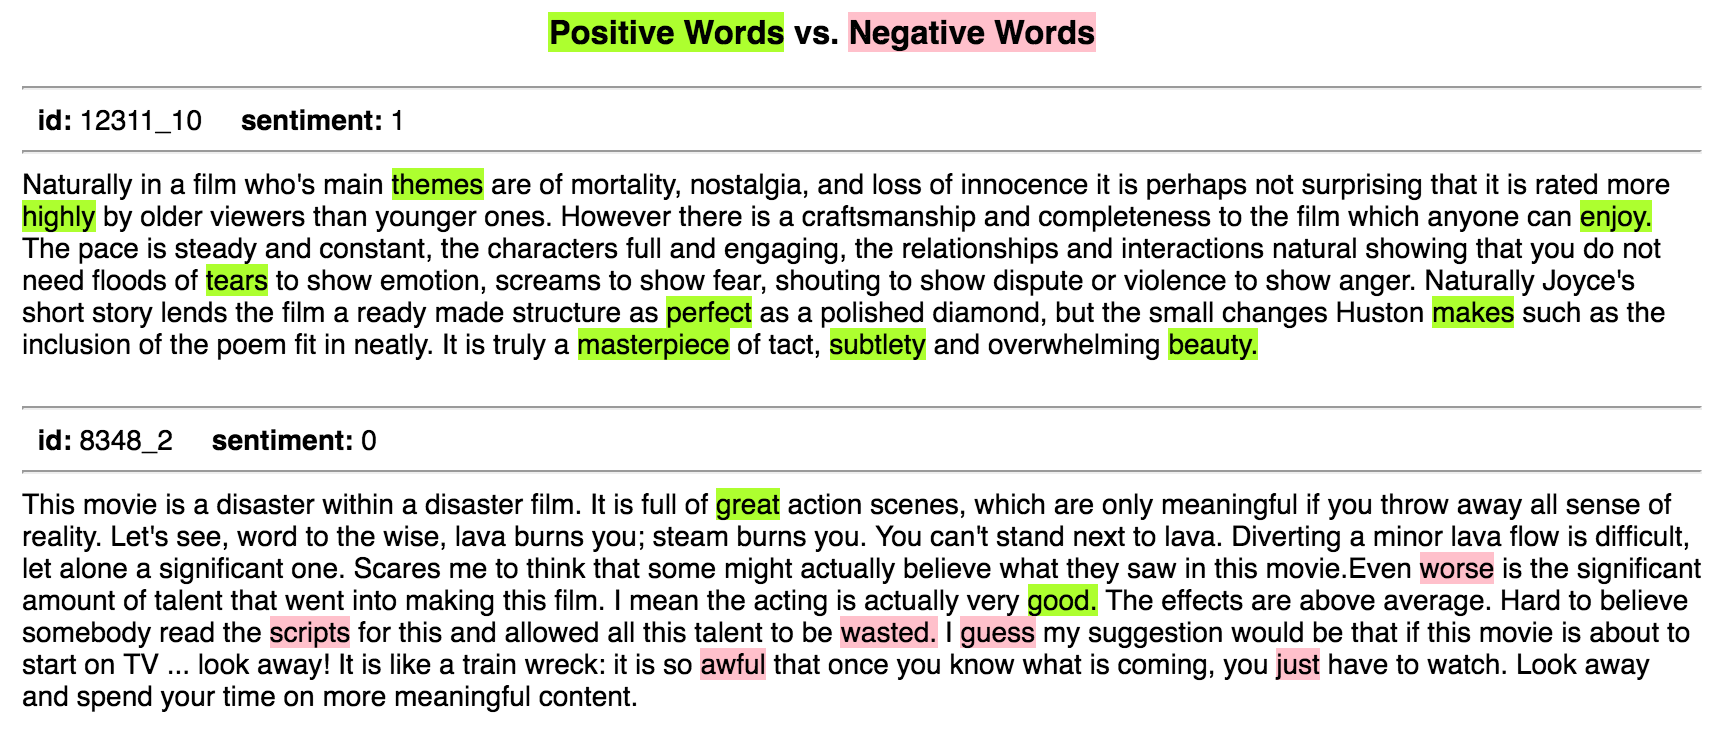
\includegraphics[width=0.72\textwidth]{example.png}
\caption{Visualization effect showing by two examples of positive/negative word labeling.} \label{fig:temp_dose}
\end{figure*}

\begin{figure*}%
    \centering
    \subfloat[Top 30 word sorted by relative word importance from Random Forest model.]{{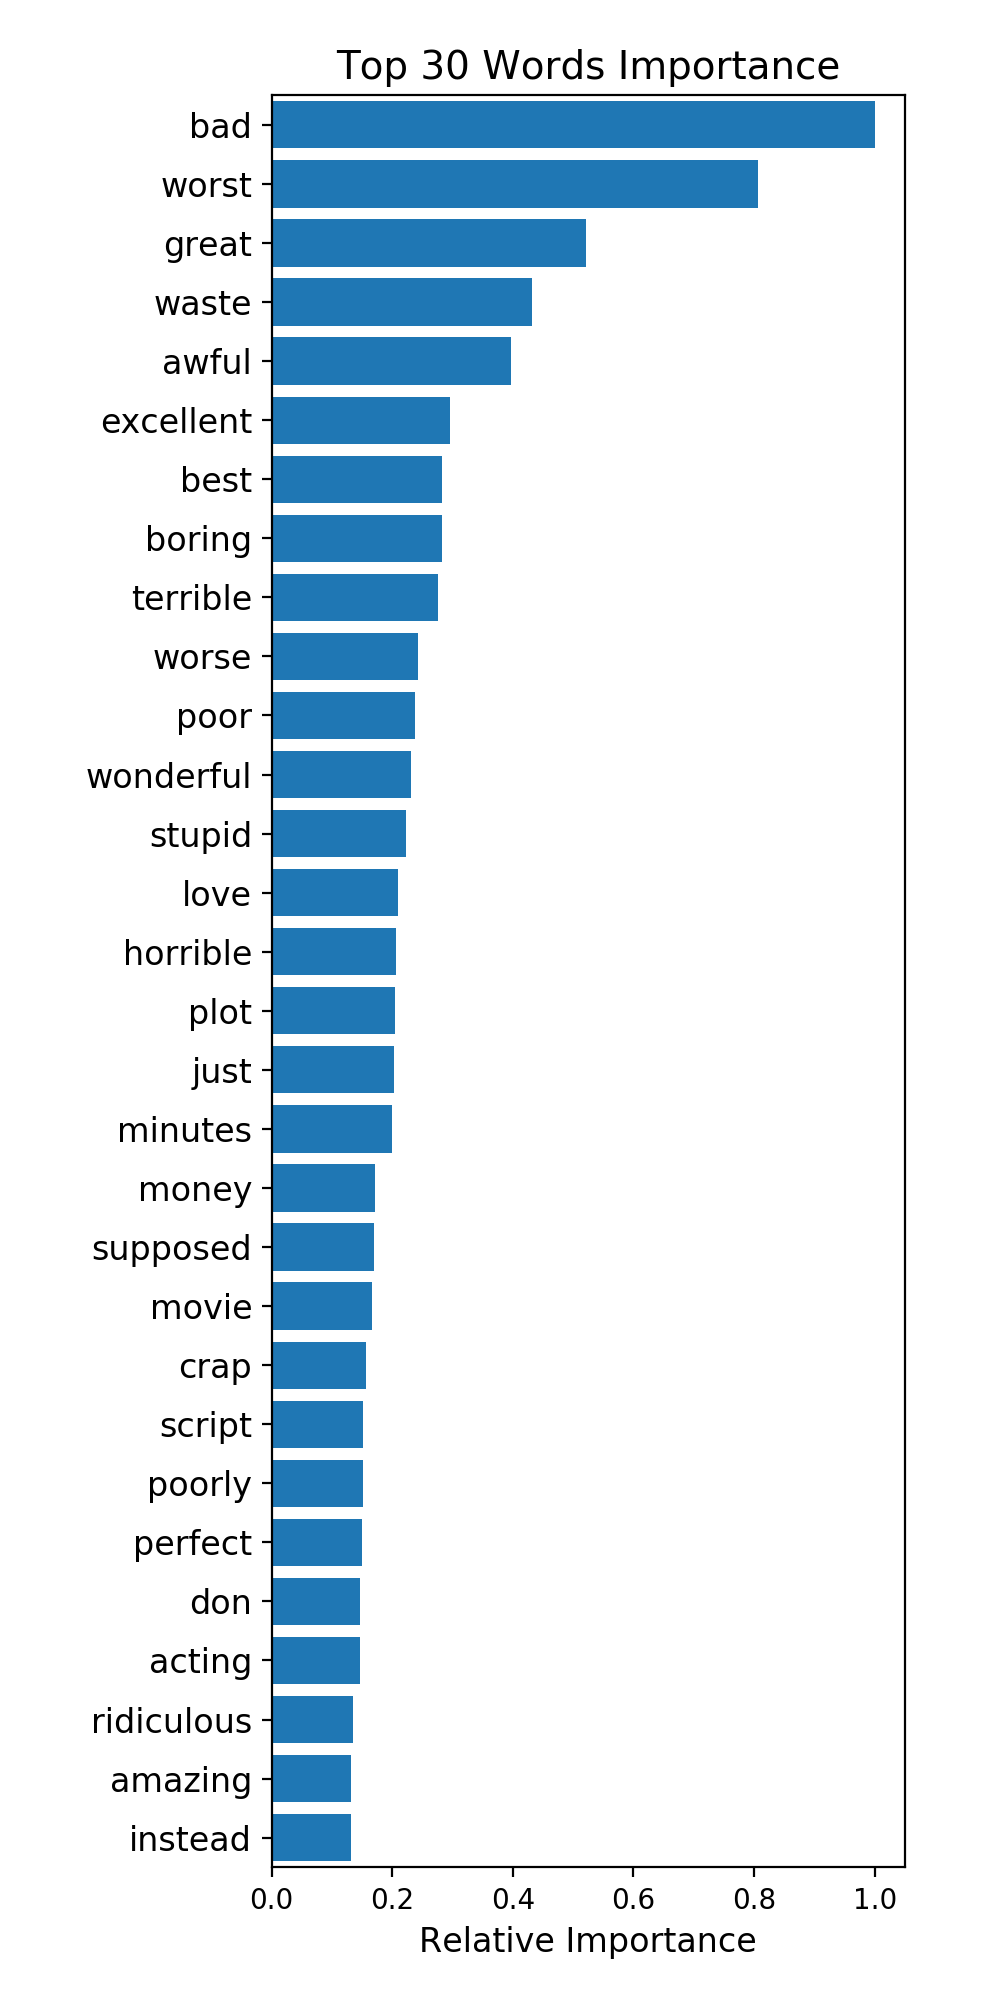
\includegraphics[width=0.4\linewidth]{importance.png} }}%
    \qquad
    \subfloat[Top 30 positive/negative words from Logistic Regression.]{{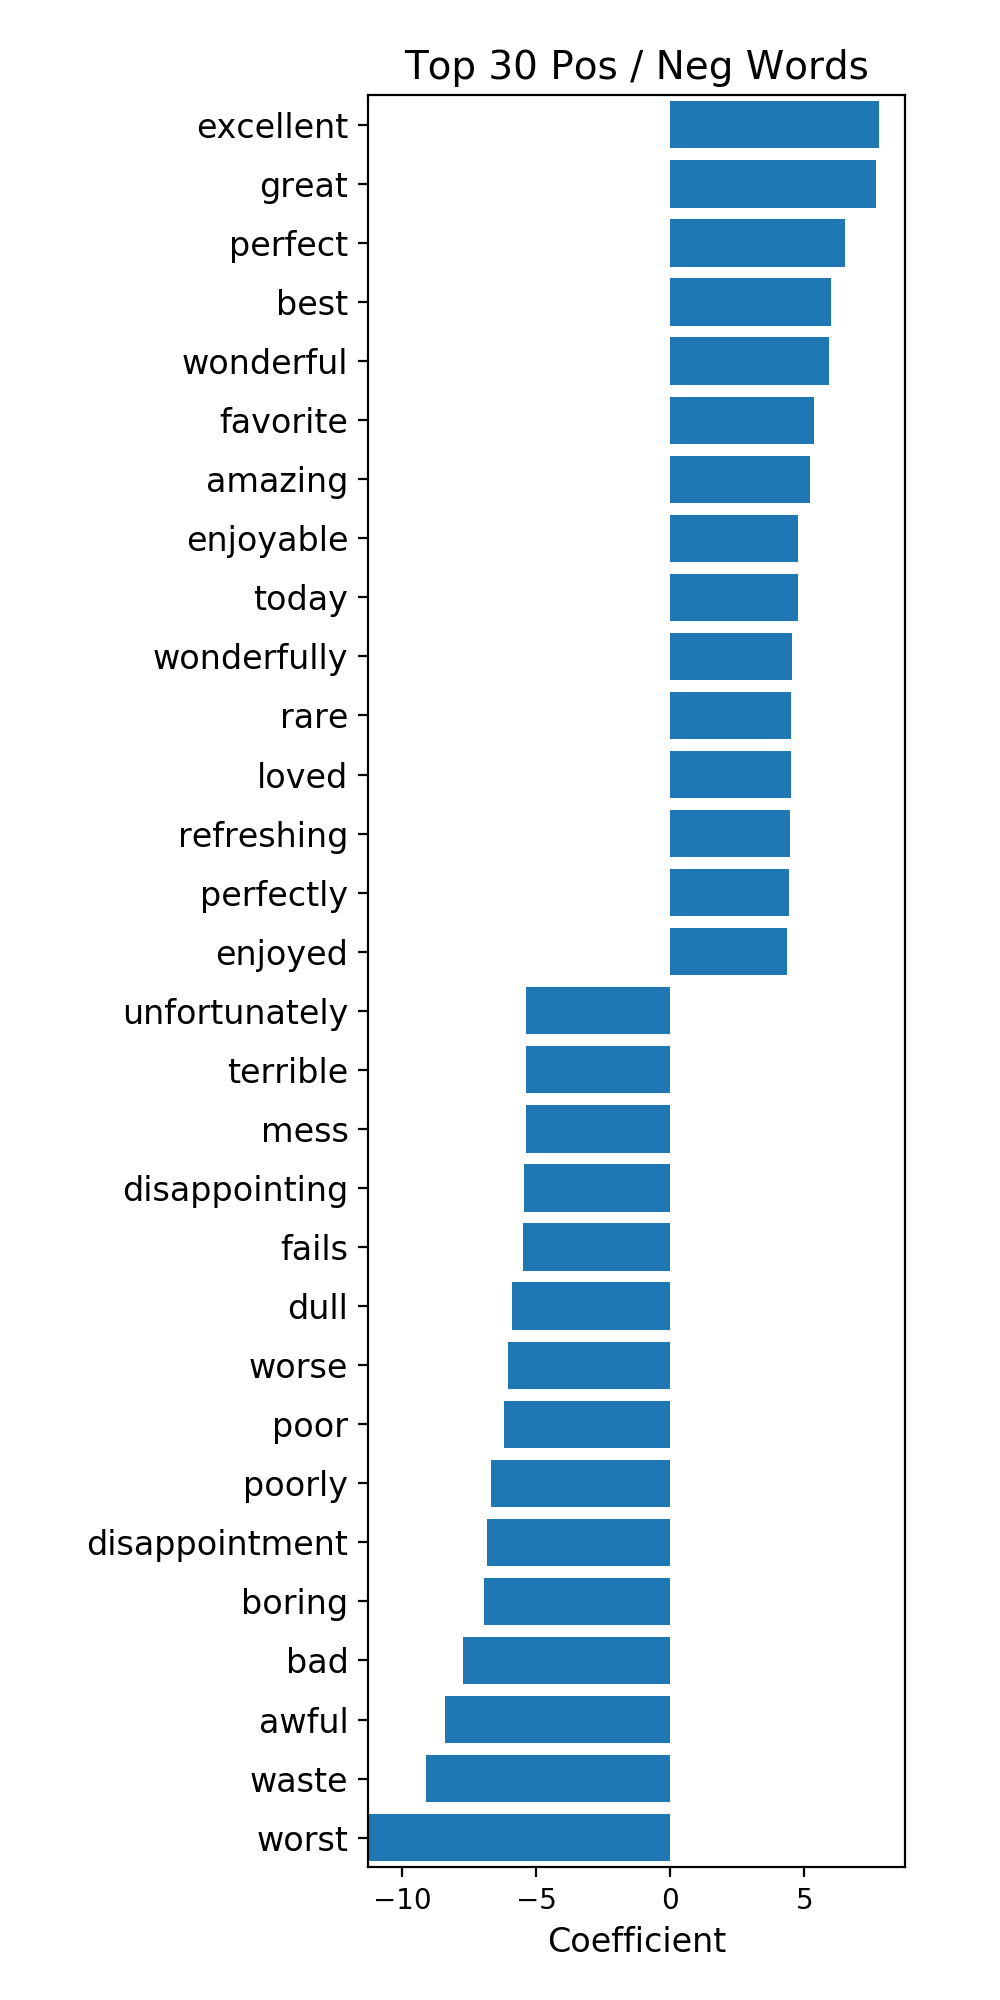
\includegraphics[width=0.4\linewidth]{top_words.png} }}%
    \caption{Visualization result from Logistic Regression and Random Forest }%
    \label{fig:example}%
\end{figure*}

% References should be produced using the bibtex program from suitable
% BiBTeX files (here: strings, refs, manuals). The IEEEbib.bst bibliography
% style file from IEEE produces unsorted bibliography list.
% -------------------------------------------------------------------------
%\bibliographystyle{IEEEbib}%\bibliography{strings,refs}
%\bibliography{strings}

\end{document}